% Paket schulschriften
% Dokumentation
% Version 1
% Walter Entenmann
% 17.10.2012, 07.11.2012
%

\documentclass[12pt,titlepage]{article}
\usepackage[T1]{fontenc}
\usepackage[ngerman]{babel}

% Metafont-Logo:
\usepackage{mflogo}
% Einbinden von eps-Files:
\usepackage{graphicx}
% Lineaturen:
\usepackage{schulschriften_lin}
% LaTeX-Anpassung, Umschaltung, Unterstreichen:
\usepackage{schulschriften_ltx}


\hoffset-1in
\voffset-1in
\textwidth160mm
\textheight250mm
\oddsidemargin25mm
\parindent0pt
\sloppy

% Zaehler bei ltx:
\newcounter{mysection}

% eps-Files der Fonttabellen als Floats:
\newcommand{\Figure}[4]{
\begin{figure}[htbp]
\unitlength1mm
\begin{picture}(160,#3)
#4
\end{picture}
\caption{#2}\label{#1}
\end{figure}}

\begin{document}

% Bild
\renewcommand{\figurename}{Bild}

% Titelseite
\title{{\huge\bfseries Dokumentation}\\[5mm]
Das \MF-Paket {\sffamily\bfseries schulschriften}\\
f\"ur die Schulausgangsschriften --\\
 von S\"utterlin bis heute}
\author{Walter Entenmann\thanks{E-mail: walter.entenmann@t-online.de}}
\date{Version 1\\5. November 2012}
\maketitle

\newpage
\section*{Zusammenfassung}
Das Paket {\sffamily schulschriften}  enth\"alt  im wesentlichen 
die \MF-Quellfiles
f\"ur die folgenden Schulausgangsschriften:
S\"utterlinschrift, Deutsche Normalschrift, 
Lateinische Ausgangsschrift, Schulausgangsschrift und 
Vereinfachte Ausgangsschrift. Dazu kommen noch
die Fontdefinitionsfiles, die Fonttabellen, 
einige Stilfiles z.B. f\"ur Lineaturen und
Beispiele sowie diese Dokumentation. 
Damit ist es m\"oglich, beliebige deutsche Texte in diesen
Schreibschriften zu schreiben.

Die Anleitung gibt  einen \"Uberblick \"uber die enthaltenenen Dateien
und beschreibt deren Installation in einem lokalen texmf-Baum im
Home-Directory.
Die Anwendung der Schreibschriften in einem \LaTeX-Dokument wird
anhand von Beispielen erl\"autert. 
Dazu geh\"ort auch das Schreiben auf ein Liniensystem und die
Umschaltung zwischen Schreibschrift und Normalschrift.
Zu allen Schriften sind die Fonttabelle und ein
Musterblatt mit allen Schriftzeichen angegeben.
Abschlie\ss{}end folgen noch  einige Bemerkungen zur historischen  Entwicklung
der Schriften.

\section{Das Paket {\sffamily schulschriften}}
Das Paket {\sffamily schulschriften} kann von CTAN \cite{11} als komprimierte
Archivdatei \verb+schulschriften.zip+ heruntergeladen werden.

Zur Vereinfachung der Darstellung ben\"utzen wir im weiteren die
folgenden Ersetzungen:\\
F\"ur den Paketnamen\\
\verb+<paket>+  $\longrightarrow$  \verb+schulschriften+\\
F\"ur die Fontnamen der S\"utterlinschrift (SU), der Deutschen
Normalschrift (DN), der Lateinischen Ausgangsschrift (LA), der
Schulausgangsschrift (SAS) und der Vereinfachten Ausgangsschrift (VA):\\
\verb+<font>+  $\longrightarrow$ \verb+wesu+ $|$ \verb+wedn+ $|$
\verb+wela+ $|$ \verb+wesa+ $|$ \verb+weva+.

Beim Entpacken der Archivdatei mit\\
\verb+unzip schulschriften.zip+ \\
im momentanen Arbeitsverzeichnis wird dort ein Unterverzeichnis
\verb+schulschriften+ ge\"offnet, welches das \verb+README+-File und die
weiteren 
Unterverzeichnisse \verb+doc+, \verb+tex+ und \verb+source+
enth\"alt. 
Nachdem man das \verb+README+-File gelesen hat, findet man im Unterverzeichnis
\verb+doc+ die  {\bfseries Dokumentation} als pdf-File.

Das Verzeichnis \verb+schulschriften+ hat insgesamt folgende Struktur:
\begin{verbatim}
.../<paket>/README
           /doc/<paket>.pdf
                <paket>.tex
           /tex/<paket>_xpl.tex
                <paket>_ltx.tex
                <paket>_lin.sty
                <paket>_ltx.sty
                <font>/t1<font>.fd
                       <font>.sty
                       <font>_fonttabelle.eps 
           /source/<font>/*.mf
\end{verbatim}

\newpage
Im einzelnen:\\
\verb+doc/+\\
Die Dokumentation des Pakets im pdf-Format  befindet sich im File
\verb+schulschriften.pdf+, das man mit dem Acrobat-Reader lesen kann:\\
\verb+acroread schulschriften.pdf+.\\
Das
zugeh\"orige \LaTeX-Quellfile \verb+schulschriften.tex+ liegt
ebenfalls bei.

\verb+tex/+\\
In diesem Unterverzeichnis sind die f\"ur alle Schriften gemeinsamen
Stil- und Beispielfiles
abgelegt. In den weiteren Unterverzeichnissen
 \verb+<font>+ befinden sich pro Schrift das
Fontdefinitonsfile, das Fontbefehlsdefinitionsfile 
und die Fonttabelle.

\verb+source/+\\
Dieses Unterverzeichnis enth\"alt pro Schrift \verb+<font>+ die eigentlichen
\MF-Quellfiles.

\section{Installation}
Damit man die Fonts in \LaTeX-Dokumenten im 
 ganzen Heimatverzeichnis
ben\"utzen kann, muss man sicherstellen, dass die ben\"otigten Quellfiles etc.
bei der \verb+latex+- und \verb+dvips+-Bearbeitung gefunden werden. 
Deshalb ist es sehr zweckm\"a\ss{}ig, die Files des Pakets
in einen lokalen \verb+texmf+-Baum im Home-Directory zu verschieben,
der bei jeder \LaTeX- und \MF-Bearbeitung automatisch durchsucht wird.
Dieser sollte folgende Struktur haben:
\begin{verbatim}
~/texmf/tex/latex/
       /fonts/source/
       /doc/
\end{verbatim}
Bevor man die Files in den \verb+~/texmf+-Baum kopiert, mu\ss{}
man sicherstellen, da\ss{} in diesem die Unterverzeichnisse 
\verb+schulschriften+ noch nicht existieren. Im Falle eines Updates
mu\ss{} man diese gegebenefalls vorher l\"oschen.

Zum Kopieren der Files geht man 
in das Verzeichnis \verb+schulschriften+, 
das beim Entpacken des Pakets entstanden ist, und gibt die Kommandos:
\begin{verbatim}
cp -r source ~/texmf/fonts/source/schulschriften
cp -r tex ~/texmf/tex/latex/schulschriften
cp doc/*.tex ~/texmf/tex/latex/schulschriften
cp doc/*.pdf ~/texmf/doc
\end{verbatim}
Zum Abschluss muss man noch das \TeX-Filesystem \verb+Kpathsea+
mit dem   Kommando\\
\verb+sudo mktexlsr+\\
aktualisieren und einmalig die Benutzerrechte anpassen gem\"a\ss{}\\
\verb+sudo chown <user>:<user> ~/texmf/ls-R+,\\
damit das Filesystem ohne root-Rechte automatisch ver\"andert werden
kann.
(F\"ur \verb+<user>+ ist der Benutzername einzusetzen.) 

Anmerkung:\\
Auf manchen Systemen gen\"ugt es statt dessen, nur das Kommando\\
\verb+mktexlsr ~/texmf+\\
zu geben.

Damit ist die Installation beendet.

Die Dokumentation erh\"alt man jetzt mit dem Befehl\\
\verb+texdoc schulschriften+.

(Auch die \LaTeX-Bearbeitung des zugeh\"origen
\verb+schulschriften.tex+-Quellfiles 
ist m\"oglich.)

\section{Die File-Hierarchie der Schriftfonts}
Die \MF-Quellfiles der einzelnen Schriften gliedern sich in
Hauptfile (Driver-File), Programfiles und
Parameterfiles.

Die \emph{Programfiles} enthalten den \MF-Programm-Code
f\"ur die einzelnen Schriftzeichen einer Schrift.

Das \emph{Hauptfile} ist das eigentliche \MF-Quellfile mit
einem Vereinbarungsteil zur Festlegung der Fontgr\"o\ss{}e,
der Federn, der Zeicheneinheit, der Transformation slanted, usw.
Es l\"adt am Ende die Programfiles und schlie\ss{}t mit \verb+end+.

Die \emph{Parameterfiles} sind sehr einfach aufgebaut. Sie setzen
lediglich einen der Steuerparameter und laden letztlich das Hauptfile.

Insgesamt ergibt sich folgende Hierarchie:
\begin{verbatim}
Parameterfiles:
<font>bsl14.mf    setzt bold=1 und laedt <font>sl14.mf   (nur SU)
<font>sl14.mf     setzt slant  und laedt das Hauptfile    
<font>b14.mf      setzt bold=1 und laedt das Hauptfile   (nur SU) 
Hauptfile:
<font>14.mf       setzt wortende=false und laedt die Programfiles
Programfiles:
<font>14_def.mf   Variable und Makros
<font>14_gr.mf    Grossbuchstaben
<font>14_kl.mf    Kleinbchstaben
<font>14_sz.mf    Satzzeichen, Ziffern, Sonderzeichen
<font>14_end.mf   siehe unten
<font>14_lig.mf   Ligaturtabellen

Parameterfile:
<font>14_end.mf   setzt wortende=true 
                  und laedt <font>14_gr.mf, <font>14_kl.mf (nicht VA)
\end{verbatim} 


\section{\MF-Bearbeitung}
In einem \LaTeX-Dokument erfolgt die Schriftauswahl mit dem Kommando\\
\verb+\usefont{T1}{<font>}{<series>}{<shape>}+\\
Dabei ist \verb+<series>+ $\longrightarrow$ \verb+m+ $|$ \verb+b+,\\
\verb+<shape>+ $\longrightarrow$ \verb+n+ $|$ \verb+sl+\\
 mit
\verb+m+ medium (Redisfeder), \verb+b+ bold (Bandzugfeder),
 \verb+n+ normal (senkrecht), \verb+sl+ slanted (geneigt).
Bold gibt es nur bei der S\"utterlinschrift.
Es k\"onnen folgende Schriften und Schnitte aus den in der folgenden
Tabelle angegebenen Quellfiles erzeugt
werden:
\begin{center}
\begin{tabular}{|l|c|c|c|c|}
\hline
&\multicolumn{4}{c|}{series}\\ 
\cline{2-5} 
&\multicolumn{2}{c|}{m (Redisfeder)} &   \multicolumn{2}{c|}{b (Bandzugfeder)}\\
\cline{2-5} 
&\multicolumn{2}{c|}{shape} & \multicolumn{2}{c|}{shape}\\
\cline{2-5} 
 Schrift & n (senkrecht)& sl (geneigt)& n  (senkrecht)& sl (geneigt)\\
\hline
SU  & \framebox{wesu14.mf} &  wesusl14.mf &  wesub14.mf  & wesubsl14.mf\\
DN  &  wedn14.mf  &  \framebox{wednsl14.mf}&&\\
LA  &  wela14.mf  & \framebox{welasl14.mf}&&\\
SAS &  wesa14.mf  & \framebox{wesasl14.mf}&&\\
VA  &  weva14.mf  &  \framebox{wevasl14.mf}&&\\
\hline
\multicolumn{5}{l}{Eingerahmt ist jeweils der Standard-Font.}
\end{tabular}
\end{center}
Die \MF-Bearbeitung erfogt mit den Shell-Kommendos\\
\verb+mf '\mode=localfont;' input <font>14+\\
\verb+mf '\mode=localfont;' input <font>sl14+\\
und bei SU zus\"atzlich\\
\verb+mf '\mode=localfont;' input wesub14+\\
\verb+mf '\mode=localfont;' input wesubsl14+


Als Ergebnis entstehen die zugeh\"origen TeX-Fontmetrikfiles \verb+*.tfm+
und die Pixelfiles \verb+*.<pixel>gf+. Letztere werden nicht weiter ben\"otigt und
k\"onnen daher gel\"oscht werden.

Im allgemeinen ist diese explizite \MF-Bearbeitung aber nicht
erforderlich,
weil
Latex die ben\"otigten   \verb+*.tfm+-Files automatisch aus den Quellfiles
\verb+*.mf+ generiert, wenn es diese findet.  Der \verb+dvips+ generiert
anschlie\ss{}end die
ben\"otigten Pixelfiles \verb+.<pixel>pk+. 
Wenn die \verb+*.mf+-Files in \verb+~/texmf/fonts/source/...+ gefunden wurden, werden die
erzeugten \verb+*.tfm+- und \verb+*.<pixel>pk+-Files in \verb+~/texmf/fonts/tfm/...+ bzw.
\verb+ ~/texmf/fonts/pk/ljfour/...+ unter gleichnamigen Unterverzeichnissen abgelegt.

\section{Anwendung in einem \LaTeX-Dokument}
\subsection{Minimalbeispiel}
Nach diesen Vorbereitungen betrachten wir nun die Anwendung der Fonts
in einem LaTeX-Dokument.
Das File \verb+schulschriften_xpl.tex+ ist ein Minimalbeispiel
und hat folgenden Aufbau
\begin{verbatim}
\documentclass{article}
\usepackage[T1]{fontenc}
\begin{document}
\usefont{T1}{wesu}{m}{n}
Ein Text in Schreibschrift.
\end{document}
\end{verbatim} 
Die
Bearbeitung mit\\
\verb+latex schulschriften_xpl+\\
\verb+dvips schulschriften_xpl+\\
\verb+gv schulschriften_xpl.ps+\\
liefert als Ergebnis

{\usefont{T1}{wesu}{m}{n} Ein Text in Schreibschrift.}

\medskip
\"Offnet man das .tex-File mit einem Editor, kann man eine andere
Schrift einstellen.


\subsection{Umlaute, scharfes s}
Es gibt zwei M\"oglichkeiten zur Eingabe der Umlaute und des scharfen
s:\\
1. Die Original \TeX-Codierung.\\
\verb+\"a+ ergibt \"a, \verb+\ss+ ergibt \ss. Z.B. 
\verb+...mit gro\ss em Eifer...+ ergibt ...mit gro\ss em Eifer...
Alle anderen Eingabevarianten funktionieren leider nicht.

2. Die direkte Eingabe auf der Tastatur.\\
Man l\"adt in der Pr\"aambel \verb+\usepackage[utf8]{inputenc}+
und gibt die Umlaute und das scharfe s direkt von der deutschen
Tastatur ein. Die Angabe \verb+utf8+ ist systemabh\"angig und
lautet u.U. \verb+latin1+, etc.

 \subsection{Schriftauswahl und -gr\"o\ss{}e, Einzug, Eurosymbol}
\noindent$\bullet$ Die \emph{Schriftauswahl} erfolgt mit dem latex-Befehl\\
\verb+\usefont{T1}{<font>}{<series>}{<shape>}+.

Optional kann man auch mit \verb+\usepackage{<font>}+
das Fontbefehlsdefinitionsfile \verb+<font>.sty+ laden
und den Schriftfont mit den dort definierten Befehlen f\"ur die
Standard-Fonts gem\"a\ss{}
\verb+\<font>+ vornehmen.

\noindent$\bullet$ Diese Stilfiles definieren auch das
\emph{Eurosymbol}, 
das man mit dem Befehl
\verb+\euros+ verwenden kann. 

\noindent$\bullet$ Die \emph{Schriftgr\"o\ss{}e} wird mit\\
\verb+\fontsize{<schriftgroesse>}{<zeilenabstand>}\selectfont+
eingestellt. Alternativ kann man auch wie \"ublich
die Schriftgr\"o\ss{}enbefehle
\verb+\large+ etc. verwenden.

\noindent$\bullet$ Damit der \emph{Einzug} zu Beginn eines jeden
Abschnitts den f\"ur die gew\"ahlte Schreibschrift ma\ss{}geblichen
Wert aufweist, muss man diesen unmittelbar nach der Schriftauswahl
einstellen mit \verb+\par\parindent1em+.


\subsection{Textbeispiele}
F\"ugt man in die Zeilen 4--5 des  Minimalbeispiels Anweisungen der Form
\begin{verbatim}
{\fontsize{16pt}{22pt}\usefont{T1}{wesu}{m}{n}
{\normalfont\normalsize\makebox[20mm][l]{SU: m n}} 
Es war ein Thema, das damals in der Luft\par}
\end{verbatim}
ein, erh\"alt man die folgenden Schriftbeispiele 
f\"ur alle Schriften und Schnitte.

{\fontsize{16pt}{22pt}\usefont{T1}{wesu}{m}{n}
{\normalfont\normalsize\makebox[20mm][l]{SU: m n}} Es war ein Thema, das damals in der Luft\par
}

{\fontsize{16pt}{22pt}\usefont{T1}{wesu}{m}{sl}
{\normalfont\normalsize\makebox[20mm][l]{SU: m sl}} Es war ein Thema, das damals in der Luft\par
}


{\fontsize{16pt}{22pt}\usefont{T1}{wesu}{b}{n}
{\normalfont\normalsize\makebox[20mm][l]{SU: b n}} Es war ein Thema, das damals in der Luft\par
}


{\fontsize{16pt}{22pt}\usefont{T1}{wesu}{b}{sl}
{\normalfont\normalsize\makebox[20mm][l]{SU: b sl}} Es war ein Thema, das damals in der Luft\par
}

{\fontsize{16pt}{22pt}\usefont{T1}{wedn}{m}{sl}
{\normalfont\normalsize\makebox[20mm][l]{DN: m sl}} Es war ein Thema, das damals in der Luft\par
}

{\fontsize{16pt}{22pt}\usefont{T1}{wela}{m}{sl}
{\normalfont\normalsize\makebox[20mm][l]{LA: m sl}} Es war ein Thema, das damals in der Luft\par
}

{\fontsize{16pt}{22pt}\usefont{T1}{wesa}{m}{sl}
{\normalfont\normalsize\makebox[20mm][l]{SAS: m sl}} Es war ein Thema, das damals in der Luft\par
}

{\fontsize{16pt}{22pt}\usefont{T1}{weva}{m}{sl}
{\normalfont\normalsize\makebox[20mm][l]{VA: m sl}} Es war ein Thema, da damals in der Luft\par
}



\section{Stilfiles}
\subsection{Stilfile f\"ur Liniensystem}
Das Stilfile \verb+schulschriften_lin.sty+ definiert folgende
\LaTeX-Befehle:\\
\verb+\Linien[breite]{text}+\\
\verb+\Zeile[breite]{text}+\\
\verb+\Linienblatt[text]{schriftgroesse}{zeilenabstand}{zeilenzahl}{breite}+\\
Vor dem Aufruf der Befehle muss man die gew\"unschte Schrift
einstellen.

Das Stilfile definiert auch die Farben \verb+hellgrau+ 
f\"ur den  Hintergrund und \verb+dunkelgrau+
f\"ur Linien. Das Schriftfeld ist wei\ss{}.
Der Befehl \verb+\Zeile+ unterscheidet sich von \verb+\Linien+
nur hinsichtlich der Farbe der Linien (dunkelgrau statt schwarz).
Ohne explizite Angabe der \verb+breite+ richtet sich diese nach der
Breite des Textes \verb+text+.
Der Befehl \verb+\Linienblatt+ beginnt eine neue Seite, stellt als
Hintergrundfarbe \verb+hellgrau+ ein, und schreibt den Text schwarz in
ein wei\ss{}es Schriftfeld.
Mit dem Befehl \verb+\color{farbe}+ unmittelbar vor \verb+text+ kann
auch eine andere Farbe f\"ur die Schrift gew\"ahlt werden, z.B.
\verb+{\color{red}text}+.


\subsubsection{Beispiel, Text auf Linien}
Die folgenden Anweisungen zeigen die verschiedenen M\"oglichkeiten,
Text in ein Liniensystem zu schreiben.
\begin{verbatim}
{\fontsize{42pt}{17mm}\usefont{T1}{wela}{m}{sl}
\Linien[\textwidth]{{\color{blue}Text auf Linien geschrieben}}

\fboxsep0pt
\Zeile[\textwidth]{{\color{red}A}}\\
\Zeile[\textwidth]{B}\\
\Zeile[\textwidth]{C}\par}
\end{verbatim}
{\fontsize{42pt}{17mm}\usefont{T1}{wela}{m}{sl}
\Linien[\textwidth]{{\color{blue}Text auf Linien geschrieben}}

\fboxsep0pt
\Zeile[\textwidth]{{\color{red}A}}\\
\Zeile[\textwidth]{B}\\
\Zeile[\textwidth]{C}
\par
}

\subsubsection{Linienblatt}
Die Formatierung eines Linienblatts f\"ur Schriftgr\"o\ss{}e 42\,pt und
Zeilenabstand 17\,mm bestehend aus 11  Zeilen der Breite 12.5\,cm,
ohne Beschriftung erfogt mit der Anweisung 
\begin{verbatim}
{\fontsize{42pt}{17mm}\usefont{T1}{wela}{m}{sl}
\Linienblatt{42pt}{17mm}{11}{12.5cm}}
\end{verbatim}
{\fontsize{42pt}{17mm}\usefont{T1}{wela}{m}{sl}
\Linienblatt{42pt}{17mm}{11}{12.5cm}
}

\subsection{Stilfile f\"ur LaTeX-Anpassung}
Wenn man  in einem \LaTeX-Dokument,  
das die Standard-Layoutbefehle \verb+\section+,\dots{}, \verb+itemize+, \verb+enumerate+, \verb+description+,
\verb+theorem+, \verb+table+, \verb+figure+, \verb+equation+ usw. verwendet, 
 als Font eine der Schreibschriften w\"ahlt,
ist man zun\"achst
entt\"auscht, weil diese Teile nicht in Schreibschrift sondern
 in Computer Modern (\TeX-Standardschrift)
gesetzt werden. Dies betrifft auch die Seitenzahlen und die
Numerierung
von Gleichungen, etc.

Das beigef\"ugte Stilfile \verb+schulschriften_ltx.sty+
ist ein Versuch, Abhilfe zu schaffen.
Es ist experimentell und vielleicht gibt es eine einfachere L\"osung. 
Bei Schreibschriften ist \underline{\strut Unterstreichen} die
 einzige Auszeichnungsm\"oglichkeit, da man ja nicht bold, italic
und verschieden gro\ss{} und schr\"ag schreiben kann.

Das Stilfile  erm\"oglicht mit den Befehlen
\verb+\normalschrift+ und \verb+\schreibschrift{<fontbefehl>}+ 
in einem \LaTeX-Dokument
das Umschalten von der \LaTeX-Standardformatierung auf die
\LaTeX-Anpassung f\"ur die verwendete Schreibschrift  und umgekehrt.
Das Kommando \verb+\schreibschrift{<fontbefehl>}+ bewirkt:\\
-- Einstellung des Fonts, z.B. \verb+<fontbefehl>+ $\longrightarrow$
 \verb+\usefont{T1}{wela}{m}{sl}+\\
-- Verwendung dieses Fonts  in \"Uberschriften (sectioning)\\
-- Setzen der Nummern  f\"ur Seitenzahlen, Gleichungen, Tabellen, Bilder
in dem eingestellten Font\\
-- In Theoremen etc. wird Fettdruck durch \underline{\strut Unterstreichen}
        ersetzt.\\
%-- Au\ss{}erdem stehen zum \uline{ein}- oder \uuline{zweifachen}
% Unterstreichen von Text 
% die Kommandos \verb+\uline{text}+ und \verb+\uuline{text}+ aus dem 
%geladenen Paket {\sffamily ulem}
% zur Verf\"ugung.
-- Im Mathematiksatz k\"onnen mit dem Befehl
\verb+\deutsch{<formelzeichen>}+ Variablen z.B. f\"ur 
Vektoren und Matrizen und die hyperbolischen Funktionen,
wie einst \"ublich, in S\"utterlinschrift gesetzt werden.
Z.B. Vektorprodukt: $\deutsch{C}=\deutsch{A}\times\deutsch{B}$.

Die praktische Anwendung zeigt das beiliegende Beispiel in
\verb+schulschriften_ltx.tex+. Die \LaTeX-Bearbeitung
\begin{verbatim}
latex schulschriften_ltx
dvips schulschriften_ltx
gv schulschriften_ltx.ps
\end{verbatim}
ergibt folgendes Ergebnis

%%%%%%%%%%%%%%%%%%%%%%%%%%%%%%%%%%%%%%%%%%%%%%%%%%%%%%%%%%%%%%%%
%%%%%%%%%%%%%%%%%%%%%%%%%%%%%%%%%%%%%%%%%%%%%%%%%%%%%%%%%%%%%%%%
\setcounter{mysection}{\value{section}}
\setcounter{section}{0}
\rule{\textwidth}{1pt}\\[-3mm]
\strut\hfill {\scriptsize Beginn des Beispiels}

\vspace{-7mm}
%%%%%%%%%%%%%%%%%%%
\schreibschrift{}\usefont{T1}{wela}{m}{sl}  %%%%%% 
\fontsize{14pt}{18pt}\selectfont\par\parindent1em
\section{\underline{\strut Lesebuch in Schreibschrift}}
\subsection{\underline{\strut Rationalit\"at im Wandel der Zeit}}
 Aber worin besteht diese wohl schon so oft
diskutierte Rationalit\"at der Vorsokratiker?
\begin{enumerate}
\item Nach der Pause, wenn's geht, wird die Besprechung 
mit den G\"asten im Seminarraum stattfinden
\end{enumerate}
\begin{description}
\item\underline{\strut Vorwort} Das Buch beginnt mit einem Vorwort, 
in welchem die Zielsetzung und der wesentliche Inhalt
\end{description}

Und jetzt schalten wir wieder auf Normalschrift um.
\normalschrift  %%%%%%
\section{Normalfont}
Und wieder ein Text in Standard-\LaTeX.
%%%%%%%%%%%%%%%%%%%%

\vspace{-3mm}
\strut\hfill {\scriptsize Ende des Beispiels}\\[-3mm]
\rule{\textwidth}{1pt}
\setcounter{section}{\value{mysection}}
%%%%%%%%%%%%%%%%%%%%%%%%%%%%%%%%%%%%%%%%%%%%%%%%%%%%%%%%%%%%%%
%%%%%%%%%%%%%%%%%%%%%%%%%%%%%%%%%%%%%%%%%%%%%%%%%%%%%%%%%%%%%%
\par\parindent0pt
\section{Besonderheiten einzelner Schriften}
\subsection{S\"utterlinschrift: Das runde s}
Eine Besonderheit der deutschen Schriften ist die unterschiedliche
Form des Buchstabens 's'. Im Prinzip  wird stets die spitze Form
'{\fontsize{12pt}{14.5pt}\usefont{T1}{wesu}{m}{n}
\symbol{179}}'
verwendet,
lediglich am Wortende steht die runde Form
'{\fontsize{12pt}{14.5pt}\usefont{T1}{wesu}{m}{n}s}', 
das sogenannte Schlu\ss-s. Dies wird in den Ligaturtabellen automatisch
ber\"ucksichtigt. Soll jedoch im Wortinneren ein 'rundes s' geschrieben
werden, z.B. bei zusammengesetzten  W\"ortern wie \verb+Hausaufgabe+, 
mu\ss{} man das 's' durch einen
nachgestellten Doppelpunkt ':' markieren, gem\"a\ss{} \verb+Haus:aufgabe+ ergibt
{\fontsize{12pt}{14.5pt}\usefont{T1}{wesu}{m}{n}
Haus:aufgabe}.
Dies hat zur Folge, da\ss{} ein echter Doppelpunkt nach einem  Wort, das auf
's' endet, verdoppelt  werden mu\ss{}. Z.B.
\verb+... besteht aus:: Holz, Stein, ...+ ergibt
{\fontsize{12pt}{14.5pt}\usefont{T1}{wesu}{m}{n}
... besteht aus:: Holz, Stein,...}

\subsection{Varianten}
Der S\"utterlin-Font enth\"alt f\"ur die Buchstaben 'I', 'J' und 'T'
auch die Varianten {\usefont{T1}{wesu}{m}{n} \'I\ \ \^I\ \ \"I\ },
die man mit \verb+\'I, \^I, \"I+ erh\"alt. Diese Formen stammen noch
aus der Kurrentschrift und wurden von S\"utterlin nicht verwendet. Man
findet sie aber h\"aufig in Handschriften aus dieser Epoche.

\subsection{Gro\ss{}e Einzelbuchstaben, Abk\"urzungen}
Gro\ss{}e Einzelbuchstaben (i.e., Gro\ss{}buchstaben am Wortende)
werden eng, aber unverbunden,  aneinander geschrieben, 
wenn sie durch ein \emph{einziges}
Leerzeichen
getrennt sind. Z.B. \verb+A\ E\ G+  ergibt 
{\fontsize{12pt}{14.5pt}\usefont{T1}{wesu}{m}{n}
A\ E\ G
}. Damit k\"onnen Abk\"urzungen sehr einfach geschrieben werden.

Sollen die Gro\ss{}buchstaben  durch ein Leerzeichen getrennt
erscheinen, mu\ss{} man \emph{zwei} explizite Leerzeichen einf\"ugen,
gem\"a\ss{}
\verb+A\ \ B\ \ C...+ ergibt
{\fontsize{12pt}{14.5pt}\usefont{T1}{wesu}{m}{n}
A\ \ B\ \ C ...
} 

Schreibt man die Buchstaben ohne Zwischenraum aneinander, werden die
verbundenen Formen verwendet, was nicht sinnvoll und
im allgemeinen unerw\"unscht sein
wird. Z.B. 
\verb+ADAC+ ergibt {\fontsize{12pt}{14.5pt}\usefont{T1}{wesu}{m}{n}
ADAC
} im Gegensatz zu \verb+A D A C + ergibt
 {\fontsize{12pt}{14.5pt}\usefont{T1}{wesu}{m}{n}
A D A C
}.

\subsection{german-Style}
Wenn man die S\"utterlinschrift verwendet, sollte man das Paket
{\sffamily babel} mit der Option \verb+german+ laden und die alten
Rechtschreib- und Trennregeln verwenden.
Au\ss{}er Umlauten gibt es bei dieser Schrift keine diakritischen
Zeichen (z.B. Akzente). Fremdsprachliche W\"orter und Texte wurden stets in
lateinischer Schrift geschrieben. 

\section{Schriftmusterseiten}
Auf Seite \pageref{p1}ff ist zu jeder Schrift ein
Musterblatt mit allen Gro\ss{}- und Kleinbuchstaben,
Ziffern und Satzzeichen abgedruckt.

Den vollst\"andigen Zeichenumfang kann man den Fonttabellen auf Seite
\pageref{p2}ff entnehmen.

Die Anweisungen zur Formatierung der Musterbl\"atter sind von der Form
\begin{verbatim}
{\fontsize{42pt}{19mm}\usefont{T1}{wesu}{m}{n}
\pagecolor{hellgrau}
\fboxsep0pt
\Zeile[\textwidth]{S\"utterlinschrift}\par
\Zeile[\textwidth]{A\ \ B\ \ C\ \ D\ \  E\ \ F\ \ 
G\ \ H\ \ I\ \ J\ }\par
...}
\end{verbatim}



\section{Fonttabellen}
\subsection{Fonttabelle erzeugen}
Mit dem New-Font-Selection-Scheme-Programm \verb+nfssfont+ kann man allgemein
zu jedem Font die zugeh\"orige Fonttabelle generieren, betrachten,
abspeichern und ausdrucken.
\begin{verbatim}
latex nfssfont
....
*<fontname eingeben, z.B. welasl14>
*\table
*\bye

dvips nfssfont
gv nfssfont.ps
\end{verbatim}
Um die korrekte  Fonttabelle f\"ur unsere Schriften zu generieren,
muss man  zuvor im Driver-File \verb+<font>14.mf+ den input-Befehl f\"ur
die Ligaturtabellen vor\"ubergehend deaktivieren.

\subsection{Die Fonttabellen der Schriften}
Auf  Seit \pageref{p2}ff sind die Fonttabellen der jeweiligen
Standard-Fonts f\"ur alle Schriften abgedruckt.

\section{Technische Daten}
Dem Entwurf der Schriften liegen folgende Daten zugrunde.

Schriftgr\"o\ss{}e, fontsize: 14pt\\
Teilungsverh\"altnis des Liniensystems: 1 : 1 : 1 (DN 2 : 3 : 2)\\
Zeicheneinheit, Einheitsl\"ange ut
\[
\mbox{ut}=\frac{\mbox{fontsize}}{\mbox{Zeicheneinheiten der Gesamth\"ohe des Liniensystems}}.
\]
Neigungswinkel $\beta$\\
Neigungsfaktor \verb+slant+\\
Anstiegswinkel des Verbindungsstrichs $\alpha^\prime$ der geneigten Schrift\\
Anstiegswinkel des Verbindungsstrichs $\alpha$ der senkrechten Schrift\\
Steigung $m$ und $m^\prime$ des Verbindungsstrichs der senkrechten
bzw. geneigten Schrift
\[
\mbox{slant}=\cot\beta,\quad m^\prime=\tan\alpha^\prime,\quad 
m=\tan\alpha=\frac{1}{\frac{1}{m^\prime}-\mbox{slant}}
\]
Exzentrizit\"at $k=b/a$,\quad $a,b$ Halbachsen der (Super-)Ellipse 
z.B. beim 'a'\\
Superness-Faktor $\sigma$.

\begin{center}
\begin{tabular}{lrrrrr}
\hline
           & SU & DN & LA & SAS & VA\\
\hline
Teilung    &1:1:1&2:3:2&1:1:1&1:1:1&1:1:1\\
$\beta$ (Grad)    & 76 & 76  & 72 & 76 & 79\\
slant      & 0.25  & 0.25 & 0.325 & 0.25 & 0.19\\
$\alpha'$ (Grad)  & 39  & 47.5& 45.25& 47.5&46.75\\
$\alpha$ (Grad)   & 45 & 56 & 56 & 56 & 53\\
$m$        & 1 & 3/2 & 3/2 & 3/2 & 4/3\\
$k$        & -- & 1.425 & 1.425 & 1.5 & 10/7\\
\hline
          &  --  &\multicolumn{4}{c}{$\sigma=0.73345$}\\
\hline
\end{tabular}
\end{center}

Strichst\"arke:\\
F\"ur Redisfeder ca. 2\% von fontsize, $d$ = 1.25ut\\
F\"ur Bandzugfeder etwa doppelt so gro\ss{},  $d$ = 2.2ut,
 Breite zu H\"ohe der Feder dx : dy
= 6 : 1, Anstellwinkel $\alpha$.
Die Strichst\"arke mit Bandzugfeder sollte f\"ur senkrechte und
geneigte Schrift gleich gro\ss{} sein 
\[
d=\mbox{dx} \sin(\beta-\alpha)
\]
Ergibt f\"ur senkrechte und geneigte Schrift dx = 3ut bzw. dx$^\prime$ = 3.5ut.

Ma\ss{}e:\\
1 \verb+em+ = fontsize = 14pt\\
1 \verb+ex+ = H\"ohe des Mittelbandes = (1/3) 14pt (DN: (3/7) 14pt)\\
1 \verb+\space+ = 1 Leerzeichen = Breite des 'n' = 25ut.

\section{Historische Entwicklung}
Abschlie\ss{}end geben wir einen kurzen \"Uberblick \"uber die historische
Entwicklung der Schreibschriften in Deutschland von S\"utterlin bis
heute \cite{12}.

\noindent$\bullet$ S\"utterlinschrift (SU)\\
Die Zeit um 1900 war gepr\"agt von tiefgreifenden Neuerungen
und Fortschritten auf allen Gebieten der Wissenschaft, Kunst und
Bildung.
Da verwundert es nicht, dass das Preu\ss{}ische Schulministerium
1911 den Graphiker  und
Dozenten an der Kunstgewerbeschule in Berlin, Ludwig S\"utterlin (1865--1917)
 damit beauftragte, eine neue deutsche
Schrift
f\"ur den Schreibunterricht an Schulen zu schaffen, die 
einfacher  ist als die seinerzeit
gebr\"auchliche Kurrentschrift (Kanzleischrift).

Die deutsche Kurrentschrift \cite{7} schreibt man
mit spitzer Feder. Sie ist stark geneigt und hat
sehr gro\ss{}e Ober- und Unterl\"angen. Durch unterschiedlichen Druck
erzielt man  haarfeine Aufstriche
und  kr\"aftige Abstriche.
Diese Schrift ist, von ge\"ubter Hand (Standesbeamte, Lehrer,
Buchhalter)
geschrieben, sehr sch\"on und
kunstvoll,
jedoch f\"ur Unge\"ubte und Sch\"uler sehr schwer zu erlernen und zu 
beherrschen.

F\"ur den Entwurf   der neuen Schreibschrift  entwickelte S\"utterlin
 die folgenden richtungsweisenden  
Ideen und Ziele, die bis heute
von Bedeutung sind \cite{1}:\\
-- Auf der Basis der deutschen Kurrentschrift, sollten unter
  Beibehaltung der prinzipiellen Buchstabenformen, diese nur
in Details vereinfacht und besser verbindbar gestaltet werden,
sodass
sie fl\"ussiger und  m\"oglichst ohne  abzusetzen, geschrieben werden
k\"onnen.
Die einzelnen Buchstaben werden etwas verbreitert.\\
-- Es sollte eine senkrecht stehende  Schrift sein, weil 
eine starke Neigung gleichf\"ormig durchzuhalten schwierig ist und zu
Verkrampfungen  f\"uhrt. \\
-- Mit der damals neu verf\"ugbaren \emph{Redisfeder (Gleichzugfeder)}
sollte das Schreiben unter Verzicht  auf unterschiedliche
Strichst\"arken  erleichtert werden.
Trotzdem hatte S\"utterlin
nichts einzuwenden, leicht geneigt 
 (z.\,B. 76 Grad)  oder mit 
einer Bandzugfeder zu schreiben, 
um eine etwas dekorativere Schrift zu erzielen.\\
-- Das Liniensystem sollte eine Aufteilung f\"ur Ober-, Mittel- und
  Unterl\"ange im Verh\"altnis 1:1:1 haben, d.h.
wesentlich geringere Ober- und Unterl\"angen als bei der
Kurrentschrift.
 Der optimale Linienabstand sollte 
gem\"a\ss{} seiner vielen praktischen Versuche
f\"ur Schulanf\"anger 5\,mm betragen. Dieses Liniensystem gilt bis
heute!

Die Einf\"uhrung der S\"utterlinschrift 
zun\"achst in Preu\ss{}en 1915  und ab 1935 allgemein, sorgte f\"ur
 eine einheitliche Basisschrift in ganz Deutschland.

Die S\"utterlinschrift wurde 1941 durch den Schrifterlass
verboten. Sie
ist  aber auch heute noch von Bedeutung f\"ur das
Lesen von Urkunden, Briefen und sonstigen Dokumenten aus dieser
Zeitepoche.
Das Kinderbuch \glqq Der Struwwelpeter\grqq{} beispielsweise ist  aktuell in
einer
S\"utterlinschrift-Ausgabe im Buchhandel erh\"altlich
 \cite{2}.

Auch in der Mathematik und in den Ingenieurwissenschaften wurden die
deutschen Schriftzeichen f\"ur Vektoren und Matrizen, 
hyperbolische Funktionen u.a. noch lange Zeit
verwendet.

\noindent$\bullet$ Deutsche Normalschrift (DN)\\
1941 wurden mit dem Schrifterlass  \cite{4}, wie bereits erw\"ahnt, 
die deutschen Schreib- und  Frakturschriften
verboten und die sogenannte \glqq  Deutsche Normalschrift\grqq{}
als lateinische Schreibschrift verordnet.
Das  Liniensystem wurde bei gleicher H\"ohe von 15\,mm jetzt
 im Verh\"altnis 2:3:2 aufgeteilt. Das Mittelband ist somit etwas
 h\"oher als die Ober- und Unterl\"ange. Die Schrift sollte mit einer
 Rechtsneigung von 75 bis 80 Grad   geschrieben werden. Der Erlass
enth\"alt eine Musterseite mit den Gro\ss{}- und Kleinbuchstaben des
Alphabets, den Ziffern  und einigen Satzzeichen.
Diese Schrift war bis 1953 an deutschen Schulen in Gebrauch.

\noindent$\bullet$ Lateinische Ausgangsschrift (LA)\\
Nach dem Krieg entwickelte der \glqq  Iserlohner Schreibkreis\grqq{}
eine neue lateinische
Schreibschrift, die
auf der Kultusministerkonferenz 1953 zur allgemeinen Schulausgangsschrift
in Deutschland erkl\"art wurde. 
Man verwendete wieder das Liniensystem von S\"utterlin.
Der Neigungswinkel betr\"agt 72 Grad  \cite{5}.

\noindent$\bullet$ Schulausgangsschrift (SAS)\\
 In der Folgezeit  wurde in der damaligen
DDR eine neue lateinische
Schreibschrift, die sogenannte \glqq Schulausgangsschrift\grqq{},
 entwickelt und dort
ab 1968 eingef\"uhrt. Eine Besonderheit dieser Schrift
stellen die Buchstaben A, F und H dar, die mit
den nachfolgenden Kleinbuchstaben knapp unter der Mittellinie fast waagrecht
verbunden werden.
Das Liniensystem bleibt unver\"andert, die Neigung betr\"agt 76 Grad.
Heute ist sie
 vorwiegend in den neuen Bundesl\"andern
in Gebrauch
\cite{6}.

\noindent$\bullet$ Vereinfachte Ausgangsschrift (VA)\\
1969 begannen auch in der BRD die Vorarbeiten f\"ur
eine neue Schreibschrift, die sogenannte \glqq Vereinfachte
Ausgangsschrift\grqq{}, die ab
1972 nach und nach eingef\"uhrt wurde. Sie basiert auf der Lateinischen
Ausgangsschrift, ist aber stark vereinfacht und funktional.
Insbesondere drei Eigenschaften sind bemerkenswert:\\
-- Die Vereinfachte Ausgangsschrift
 verwendet als erste und einzige lateinische Schreibschrift
das \glqq K\"opfchen-e\grqq{} anstelle der Schleifchen-e, sodass
 \glqq alle Buchstaben  auf der
Mittellinie beginnen und enden\grqq{}, wenn man den Verbindungsstrich
mit einbezieht.\\
Dies erleichtert nicht nur das Schreibenlernen, sondern vereinfacht
auch die Implementierung in \MF{} entscheidend.\\
--  Die Gro\ss{}buchstaben B, D, J, N, O, P, S, T,
V und W  
werden  nicht verbunden.

Das Liniensystem bleibt unver\"andert und die
Neigung betr\"agt 79 Grad \cite{5}.

Insgesamt stehen heute in Deutschland f\"ur den Schreibunterricht
drei lateinische Schriften mit einheitlichem Liniensystem 
zur Verf\"ugung, die \glqq Lateinische
Ausgangsschrift\grqq{}, die \glqq Schulausgangsschrift\grqq{} und die \glqq Vereinfachte Ausgangsschrift\grqq{}.
Die Verwendung dieser drei Schriften ist in den einzelnen
Bundesl\"andern
in unterschiedlicher Weise geregelt.

\section{Anmerkungen}
Bei der S\"utterlinschrift gibt es au\ss{}er Umlauten keine
diakritischen Zeichen. Ich habe aber bislang auch 
f\"ur die lateinischen Schriften
 keine weiteren diakritischen Zeichen entworfen,
weil man bei Schulausgangsschriften annehmen kann, dass sie
von  Schulanf\"angern im Schreibunterricht  verwendet und
 nur deutsche Texte damit geschrieben werden. 

Bei Bedarf bin ich aber gerne bereit,
den  Schriften weitere gew\"unschte  Zeichen hinzuzuf\"ugen.

\medskip
F\"ur 
Fehlermeldungen und Verbesserungsvorschl\"age, die sich aus der
praktischen Anwendung ergeben, w\"are ich daher sehr dankbar. 

%
\begin{thebibliography}{99}
\bibitem{1}
Ludwig S\"utterlin:
Neuer {L}eitfaden f\"ur den {S}chreibunterricht.
Albrecht-D\"urer-Haus,
Berlin,
1926.
\bibitem{2}
Heinrich Hoffmann:
Der {S}truwwelpeter -- ({A}usgabe in
 {S}\"utterlinschrift).
Edition Tintenfa\ss{},
Neckarsteinach,
2009.
%\bibitem{3}
%Karl Popper:
%Lesebuch.
%J.C.B. Mohr,
%T\"ubingen,
%1995.
\bibitem{4}
Schrifterlass 1941.
 www.hbf.dipf.de/cgi-shl/digibert.pl?id=BBF0833246.
\bibitem{5}
Bildungsplan {G}rundschule 2004,
  {S}.\,52.
Baden-W\"urttemberg Ministerium f\"ur Kultus, Jugend und Sport.
\bibitem{6}
Lehrplan {G}rundschule {D}eutsch 2004, 2009, {S}.\,46.
S\"achsisches Staatsministerium f\"ur Kultus.
\bibitem{7}
M. F. Eisenlohr:
Fibel -- {D}eutsches {K}inderb\"uchlein.
Ludwig Auer Verlag,
Donauw\"orth,
1998,
2. Aufl., Erstausgabe 1920.
%\bibitem{8}
%Donald E. Knuth:
%The METAFONTbook.
%Addison-Wesley,
%Reading, MA,
%1986.
%\bibitem{9}
%Helmut Kopka:
%\LaTeX{} Band 2: Erg\"anzungen -- mit einer Einf\"uhrung in \MF.
%Addison-Wesley,
%Bonn,
%1995.
%\bibitem{10}
%Walter Entenmann:
%Ein \MF-Paket f\"ur die S\"utterlinschrift.
%DANTE-Tagung Bremen,
%M\"arz 2011.
\bibitem{11}
Walter Entenmann:
Package schulschriften.
CTAN: \verb+/fonts/schulschriften+, 30.10.2012.
\bibitem{12}
Walter Entenmann:
Schulschriften -- von S\"utterlin bis heute.
Die \TeX nische Kom\"odie,
{\bfseries 24}
(2012)
4,
29--57.
\end{thebibliography}

% SU Font-Musterseite 
\newpage
\label{p1}
{
\fontsize{42pt}{19mm}\usefont{T1}{wesu}{m}{n}
\pagecolor{hellgrau}
\fboxsep0pt
\Zeile[\textwidth]{S\"utterlinschrift}\par
\Zeile[\textwidth]{A\ \ B\ \ C\ \ D\ \  E\ \ F\ \ G\ \ H\ \ I\ \ J\ }\par
\Zeile[\textwidth]{K\ \ L\ \ M\ \ N\ \ O\ \ P\ \ Q\ \ R\ \ S\ }\par
\Zeile[\textwidth]{T\ \ U\ \  V\ \ W\ \ X\ \ Y\ \ Z\ }\par
\Zeile[\textwidth]{\"A\ \ \"O\ \  \"U\ \ St\ \ \'I\ \   \^I\ \  \"I\ }\par
\Zeile[\textwidth]{a b c d e f g h i j k l }\par
\Zeile[\textwidth]{m n o p q r \ss{}  \symbol{179}\ s t }\par
\Zeile[\textwidth]{u v w x y z \"a \"o \"u }\par
\Zeile[\textwidth]{0 1 2 3 4 5 6 7 8 9 ! ?}\par
\Zeile[\textwidth]{. , ; : ' \glqq{} \grqq{} 
\flq{} \frq{} \flqq{} \frqq{}  - --}\par
\Zeile[\textwidth]{ --- + < > = / ( ) [ ]}\par
\Zeile[\textwidth]{* \% \& \S{} \# \$ @ %\euros 
}\par
}

\newpage
% DN-Font-Musterseite 
{
\fontsize{42pt}{19mm}\usefont{T1}{wedn}{m}{sl}
\pagecolor{hellgrau}
\fboxsep0pt
\Zeile[\textwidth]{Dt. Normalschrift}\par
\Zeile[\textwidth]{A B C D E F G H I J}\par
\Zeile[\textwidth]{K L M N O P Q R S}\par
\Zeile[\textwidth]{T U V W X Y Z}\par
\Zeile[\textwidth]{\"A \"O \"U \ss{} \"a \"o \"u }\par
\Zeile[\textwidth]{a b c d e f g h i j}\par
\Zeile[\textwidth]{k l m n o p q r}\par
\Zeile[\textwidth]{s t u v w x y z}\par
\Zeile[\textwidth]{0 1 2 3 4 5 6 7 8 9}\par
\Zeile[\textwidth]{( ) ' . , : ; - ! ? \glqq{} \grqq{}}\par
\Zeile[\textwidth]{/ * [ ] @ +  -- ---  < = > }\par
\Zeile[\textwidth]{\frq{} \flq{} 
  \frqq{} \flqq \S{} \$ \# \& %\euros
}\par
}

\newpage
% LA Font-Musterseite 
{
\fontsize{42pt}{19mm}\usefont{T1}{wela}{m}{sl}
\pagecolor{hellgrau}
\fboxsep0pt
\Zeile[\textwidth]{Lateinische Ausgangsschrift}\par
\Zeile[\textwidth]{A B C D E F G H I J}\par
\Zeile[\textwidth]{K L M N O P Q R S}\par
\Zeile[\textwidth]{T U V W X Y Z}\par
\Zeile[\textwidth]{\"A \"O \"U \ss{} \"a \"o \"u }\par
\Zeile[\textwidth]{a b c d e f g h i j}\par
\Zeile[\textwidth]{k l m n o p q r}\par
\Zeile[\textwidth]{s t u v w x y z}\par
\Zeile[\textwidth]{0 1 2 3 4 5 6 7 8 9}\par
\Zeile[\textwidth]{( ) ' . , : ; - ! ? \glqq{} \grqq{}}\par
\Zeile[\textwidth]{/ * [ ] @ +  -- ---  < = > }\par
\Zeile[\textwidth]{\frq{} \flq{} 
  \frqq{} \flqq \S{} \$ \# \& %\euros
}\par
}

\newpage
% SAS-Font-Musterseite 
{
\fontsize{42pt}{19mm}\usefont{T1}{wesa}{m}{sl}
\pagecolor{hellgrau}
\fboxsep0pt
\Zeile[\textwidth]{Schulausgangsschrift}\par
\Zeile[\textwidth]{A B C D E F G H I J}\par
\Zeile[\textwidth]{K L M N O P Q R S}\par
\Zeile[\textwidth]{T U V W X Y Z}\par
\Zeile[\textwidth]{\"A \"O \"U \ss{} \"a \"o \"u }\par
\Zeile[\textwidth]{a b c d e f g h i j}\par
\Zeile[\textwidth]{k l m n o p q r}\par
\Zeile[\textwidth]{s t u v w x y z}\par
\Zeile[\textwidth]{0 1 2 3 4 5 6 7 8 9}\par
\Zeile[\textwidth]{( ) ' . , : ; - ! ? \glqq{} \grqq{}}\par
\Zeile[\textwidth]{/ * [ ] @ +  -- ---  < = > }\par
\Zeile[\textwidth]{\frq{} \flq{} 
  \frqq{} \flqq \S{} \$ \# \& %\euros
}\par
}

\newpage
% VA-Font-Musterseite 
{
\fontsize{42pt}{19mm}\usefont{T1}{weva}{m}{sl}
\pagecolor{hellgrau}
\fboxsep0pt
\Zeile[\textwidth]{Vereinfachte Ausgangsschrift}\par
\Zeile[\textwidth]{A B C D E F G H I J }\par
\Zeile[\textwidth]{K L M N O P Q R S }\par
\Zeile[\textwidth]{T U V W X Y Z \"A \"O \"U}\par
\Zeile[\textwidth]{a b c d e f g h i j k l }\par
\Zeile[\textwidth]{m n o p q r s t}\par
\Zeile[\textwidth]{u v w x y z \"a \"o \"u }\par
\Zeile[\textwidth]{\ss{} st tz \ss t}\par
\Zeile[\textwidth]{0 1 2 3 4 5 6 7 8 9}\par
\Zeile[\textwidth]{! ? . , ; : '  + - < > = }\par
\Zeile[\textwidth]{/ ( ) [ ] * \% \& \S{} \# @}\par
\Zeile[\textwidth]{\glqq{} \grqq{} \flq{} \frq{} \flqq{} \frqq{}  --
  --- %\euros
}\par
}


\Figure{f1}{Fonttabelle der S\"utterlinschrift
  wesu14.\pagecolor{white}}{220}{\put(0,0){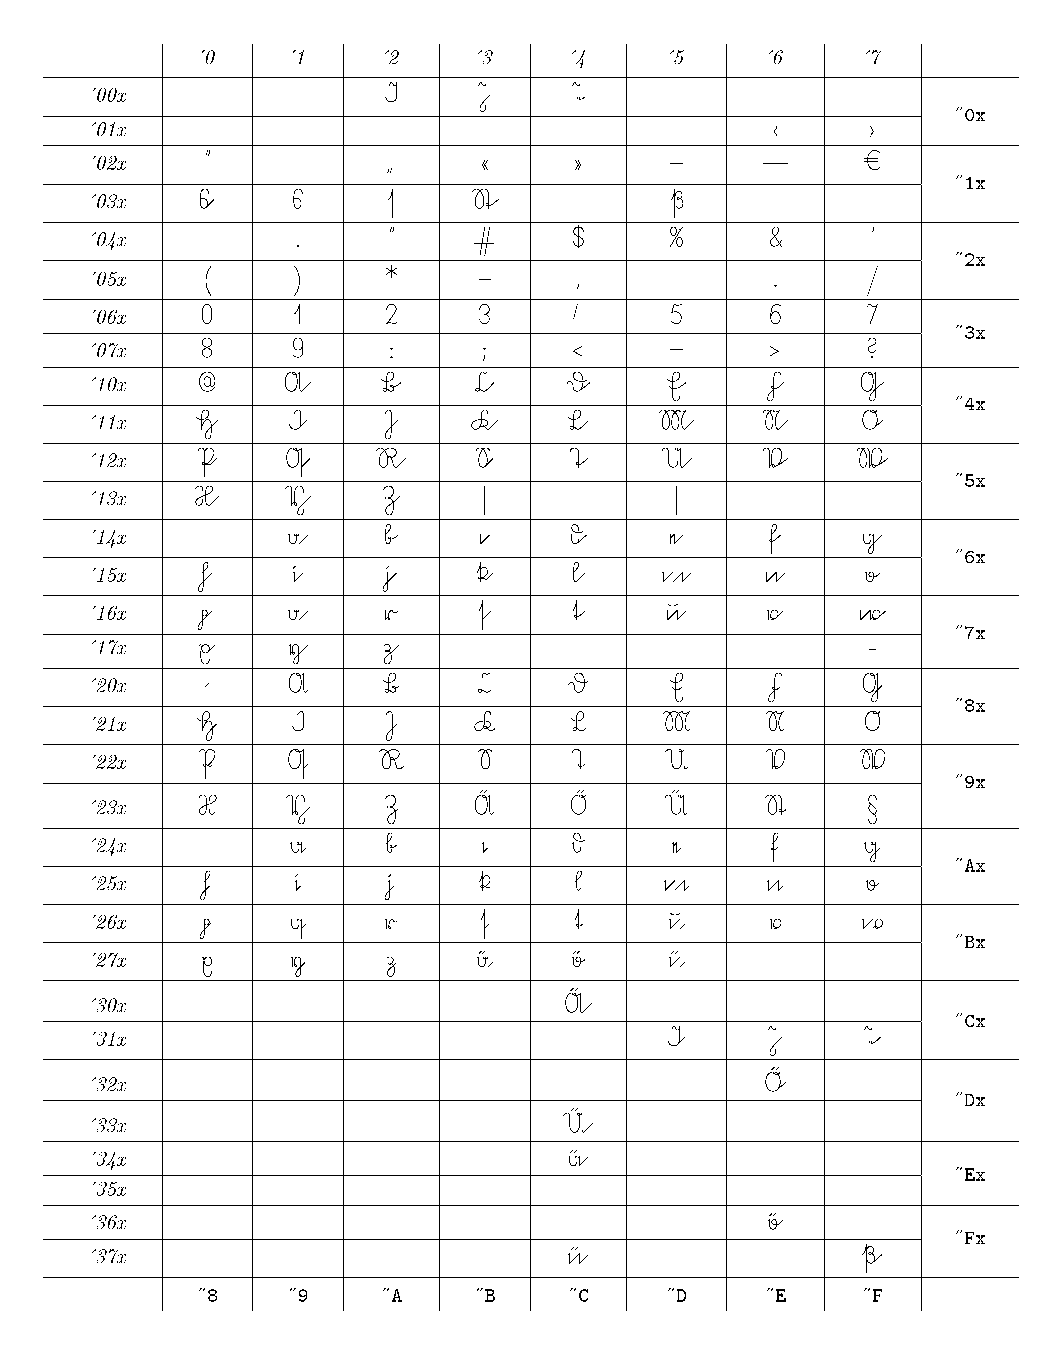
\includegraphics{wesu_fonttabelle.eps}}\label{p2}}

\Figure{f2}{Fonttabelle der Deutschen Normalschrift 
  wednsl14.}{220}{\put(0,0){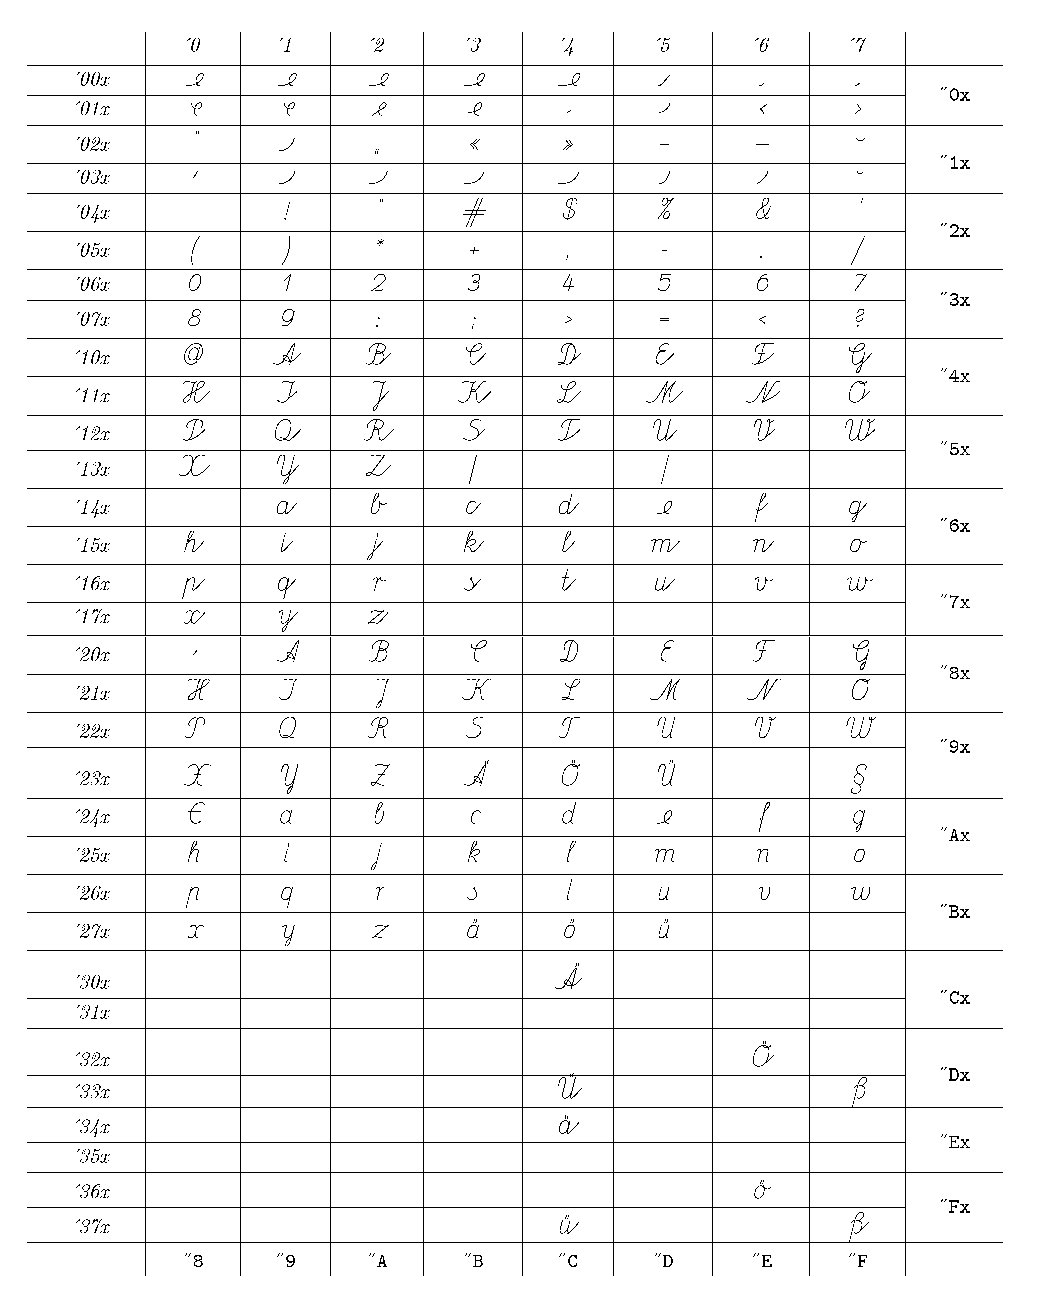
\includegraphics{wedn_fonttabelle.eps}}}

\Figure{f3}{Fonttabelle der Lateinischen Ausgangsschrift
welasl14.}{220}{\put(0,0){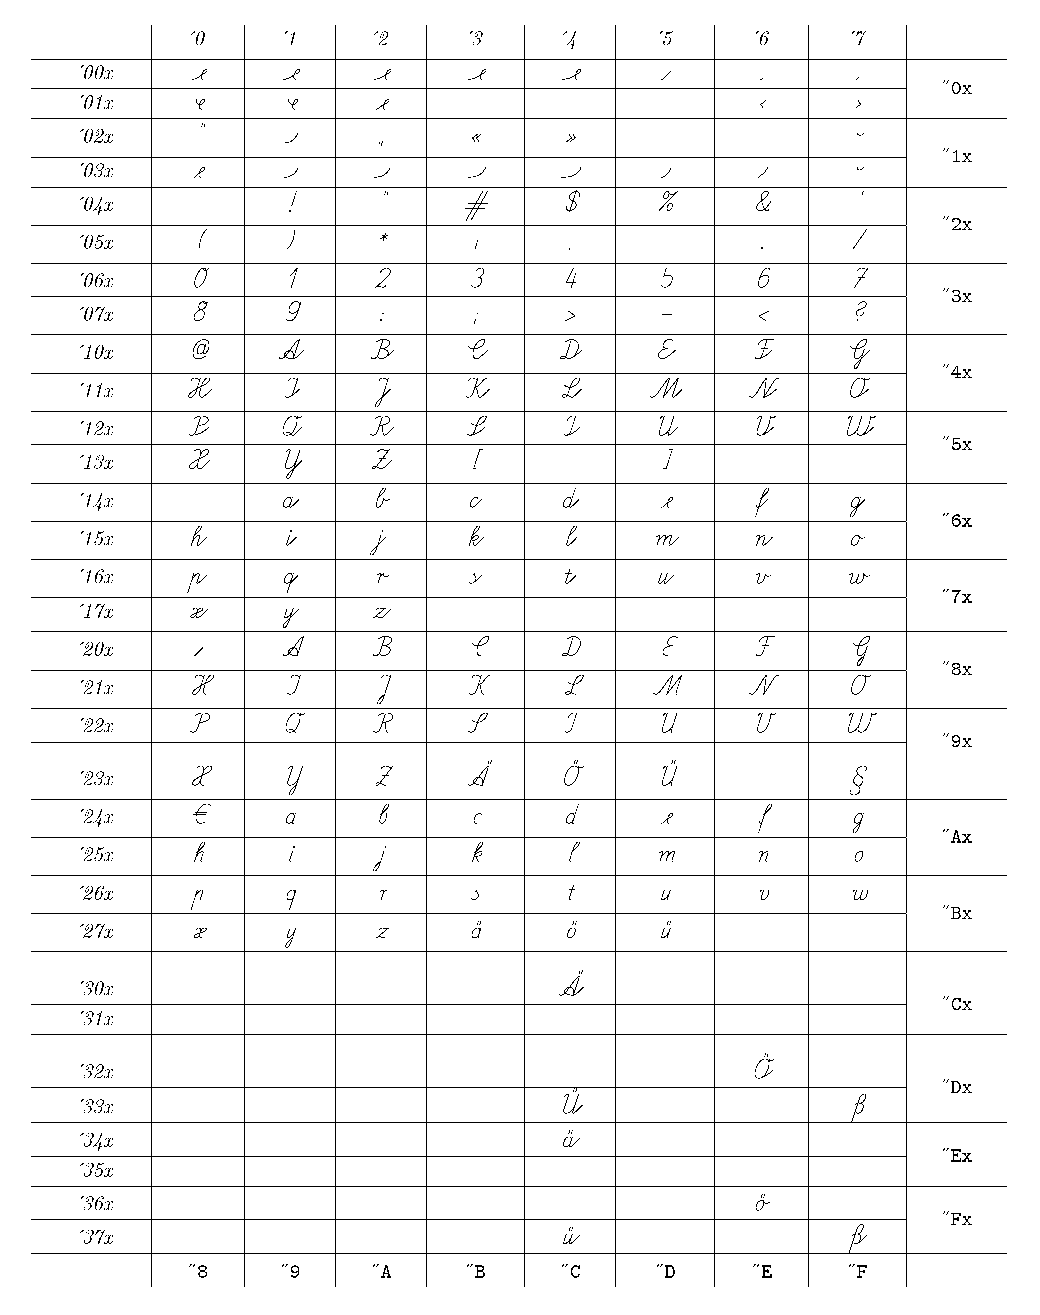
\includegraphics{wela_fonttabelle.eps}}}

\Figure{f4}{Fonttabelle der Schulausgangsschrift
wesasl14.}{220}{\put(0,0){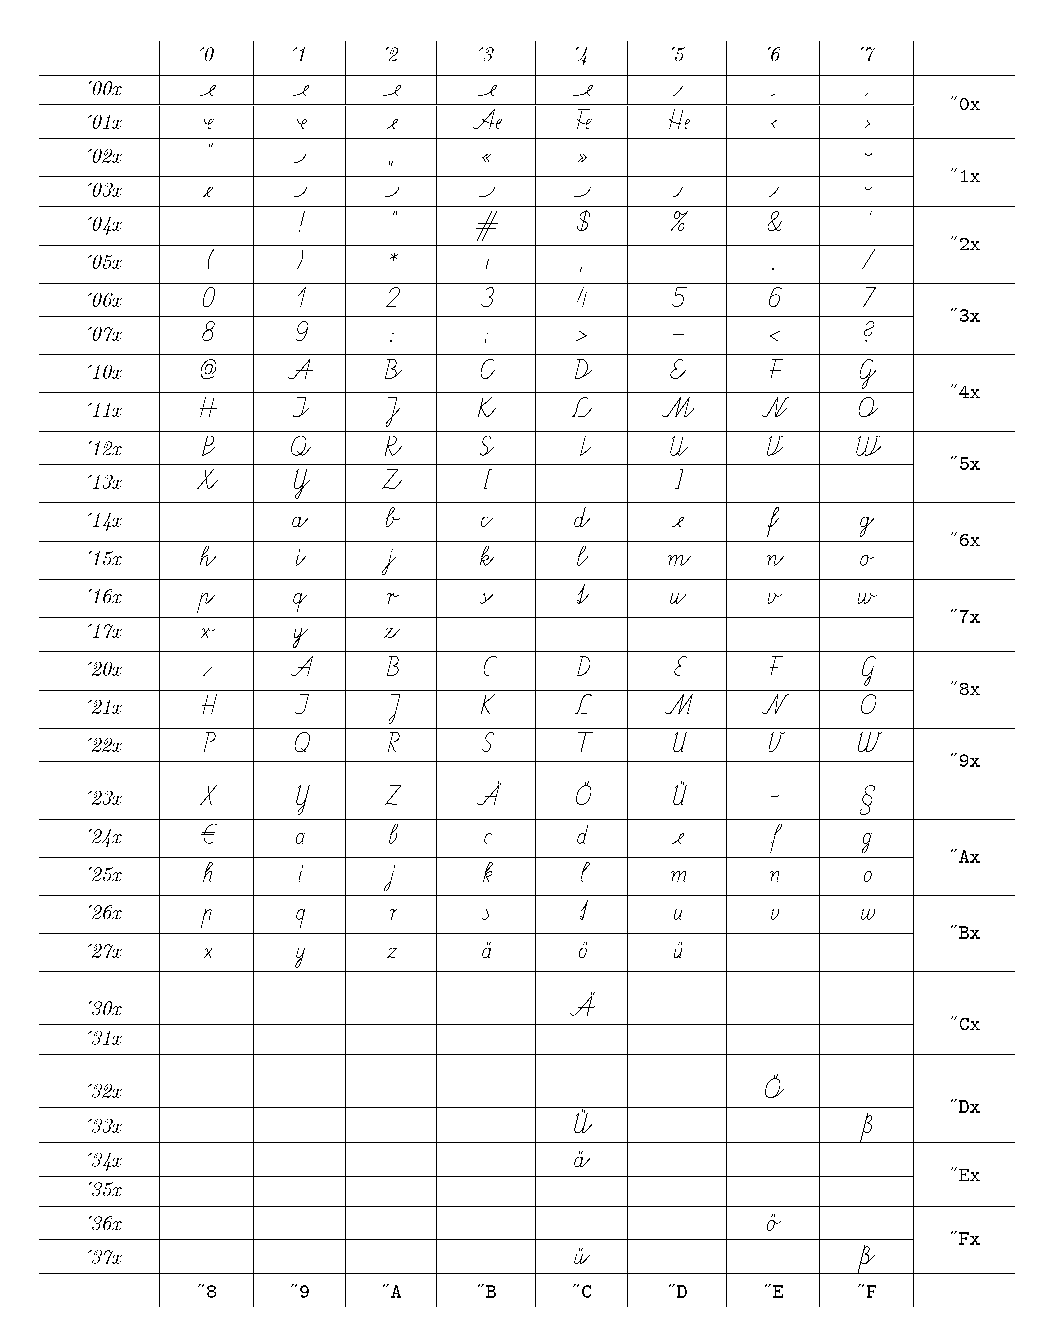
\includegraphics{wesa_fonttabelle.eps}}}

\Figure{f5}{Fonttabelle der Vereinfachten Ausgangsschrift 
wevasl14.}{190}{\put(0,0){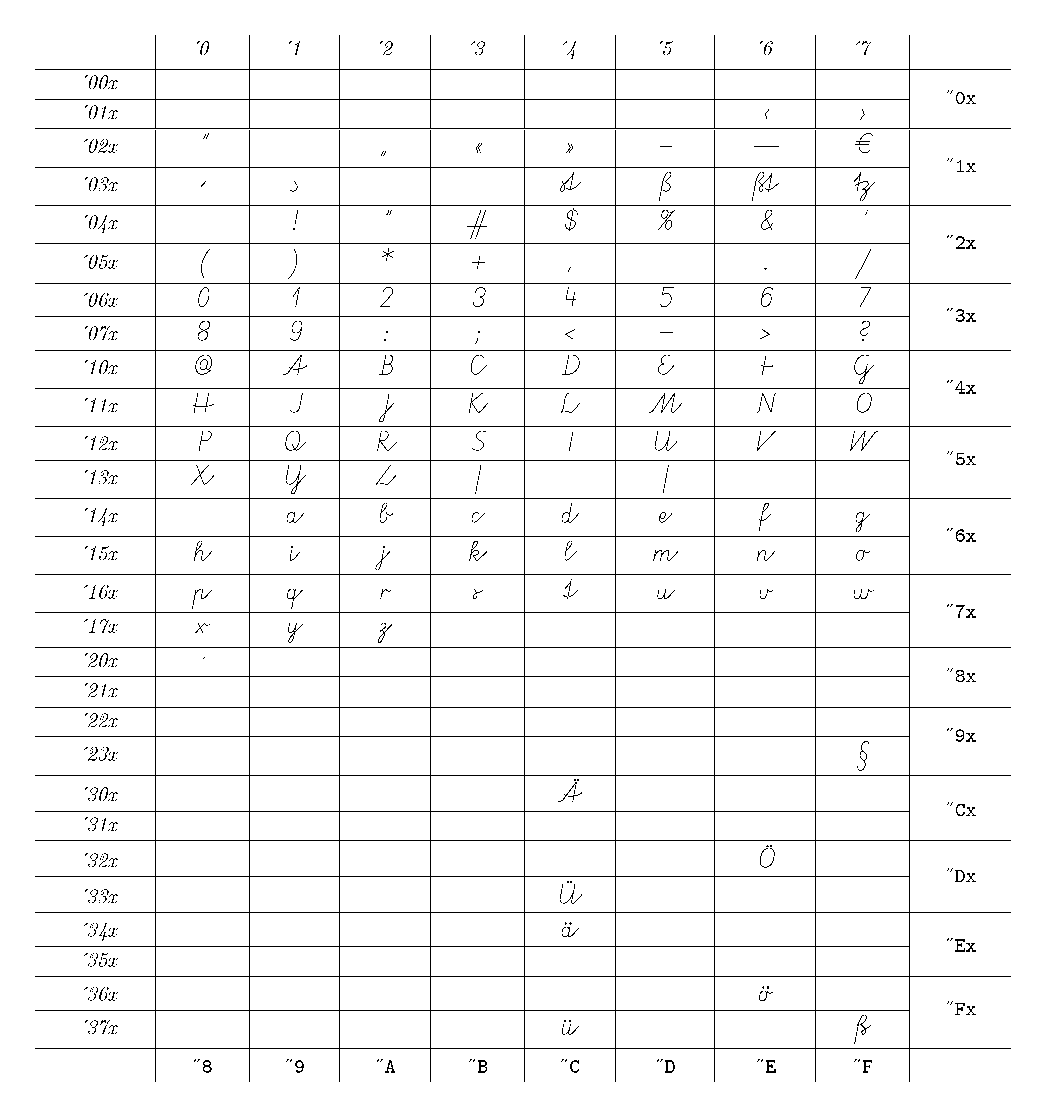
\includegraphics{weva_fonttabelle.eps}}}

\end{document}
